\section{Learning process}


% ----------------------- paths to graphics ------------------------



% ----------------------- contents from here ------------------------
% 

TODO-1: brief description and diagram of a compression learning algorithm

\subsection{Optimization problem}
\label{subsec:learningprocess:optimizationproblem}


% ----------------------- paths to graphics ------------------------



% ----------------------- contents from here ------------------------
% 

We can define the learning process as follows: given a sample from a dataset, its schema and a set of pattern detectors as input, output a compression tree that, when applied to the dataset, produces a compressed representation of it of minimum disk size.

The schema is a list of columns and their data types. The pattern detectors are implementations of the \nameref{subsec:genericpd}---receives the columns as input, evaluates the sample and returns a list of \textit{(expression node, evaluation result)} tuples. Adding an \textit{expression node} to the compression tree means: 1) altering the schema by deleting existing columns and creating new ones; 2) altering the sample by applying the \textit{compression operator} to the input columns and generating new data. The learning process can go on by recursively feeding the new schema and sample data to the pattern detectors, resulting in new \textit{(expression node, evaluation result)} tuples. This recursive process stops when no pattern detector outputs any result anymore---no pattern matches on the current schema and data.

Choosing to add or not an \textit{expression node} to the compression tree generates a new solution. This leads to a total number of \(2^n\) possible solutions (different compression trees), where \(n\) is the total number of \textit{expression nodes} generated by the recursive process (\(n\) binary decisions: \(1\) means adding a node and \(0\) not adding it). The total number of \textit{expression nodes} (\(n\)) depends on how well pattern detectors match on the initial columns and the newly generated ones. This is entirely dependent on the characteristics of the data and the patterns that were evaluated on it. In the worst case, all pattern detectors will match on any column, leading to the following expression for \(n\):
\begin{equation}
\label{eq:optimizationproblem:n}
    n = c_{in} \times (p \times \mathit{avg}(n_{p}) \times b) ^ h
\end{equation}
\begin{equation}
\label{eq:optimizationproblem:b}
    b = \mathit{avg}(c_{out})
\end{equation}
where:
\begin{itemize}
    \item[] \(n\) = total number of expression nodes
    \item[] \(c_{in}\) = number of input columns
    \item[] \(p\) = number of pattern detectors
    \item[] \(n_{p}\) = number of expression nodes returned by a pattern detector
    \item[] \(b\) = branching factor of the compression tree
    \item[] \(h\) = height of the compression tree
    \item[] \(c_{out}\) = number of output columns of an expression node
\end{itemize}

The score of each solution is given by the size of the compressed data that resulted after applying the compression tree to the dataset. The goal of the learning process is to choose the one that gives the smallest size.

The computational effort needed for each individual \textit{expression node} consists of: 1) applying the compression operator on its input columns to generate the new data (feeding each tuple in the sample data to the operator); 2) evaluating the pattern detectors on all the new columns (feeding each tuple in the sample data to each pattern detector). Moreover, some pattern detectors may need to evaluate combinations of columns instead of individual columns, which requires all the existing columns to be reevaluated for every newly generated column (e.g. \nameref{subsec:pd:columncorrelation} evaluates all pairs of 2 columns to determine the correlation coefficient between them).

\iffalse
TODO:
better formalize problem
https://en.wikipedia.org/wiki/Optimization\_problem
\fi

% ---------------------------------------------------------------------------
% ----------------------- end of thesis sub-document ------------------------
% ---------------------------------------------------------------------------

\subsection{Cost model: compression estimators}
\label{sub:estimators}

% ----------------------- paths to graphics ------------------------



% ----------------------- contents from here ------------------------
% 

The compression learning process is an optimization problem (\ref{subsec:learningprocess:optimizationproblem}) for finding the best compression tree in terms of disk size of the resulting physical columns. Solving the optimization problem requires a way to compare its solutions, i.e. estimating the final size of the compressed data. For this purpose we created a cost model which relies on leaf compression schemes size estimators (DICT, RLE, FOR, no compression) to predict the size of a column if compressed with these methods.

\textbf{Methodology}. The score of a solution (compression tree) is computed through the following methodology: 1) represent the sample data according to the compression nodes; 2) for each column of the new representation, estimate its size if it were compressed with: DICT, RLE, FOR or not compressed at all; 3) choose the smallest size among those. The result of this process is the smallest size of the new data representation if it were compressed with leaf compression schemes.

\textbf{System assumptions}. The size on disk of a compressed column depends on: 1) implementation of the compression method; 2) characteristics of the underlying database system. The former is described in the next sections as part of the estimator implementations. For the latter we defined some assumptions of the underlying system as follows:\\
a) \textit{data types}: strings are stored with null terminator, therefore their size is given by the number of characters + 1. For all other data types we consider the sizes used by Ingres Vectorwise \cite{zukowski2012vectorwise,actianingres}. \\
b) \textit{null handling}: we consider the same approach  used by Vectorwise \cite{zukowski2012vectorwise}: do not store null values, instead, keep track of their positions using a bitmap. This results in 1 additional bit for every attribute (for nullable columns).\\
c) \textit{exception handling}: we consider a whitebox approach: for each logical column store exceptions on a separate physical nullable column. The exception column has the same datatype as the logical column.

An additional assumption that we make about the underlying system is that it supports block-level compression, i.e. every block of data is compressed independently. This allows different compression schemes to be used on the same column, enabling the possibility to exploit local data characteristics.

\subsubsection{Generic compression estimator}
\label{subsub:estimator:generic}
A compression estimator takes as input a column and two samples of data (\textit{train} and \textit{test} sample) and outputs the estimated size of the compressed column. The result can be either the size of the compressed sample or the size extrapolated to the total size of the block or column. The latter requires an additional parameter specifying the total number of rows in the full data.

The estimated size has 4 components (exemplified for Dictionary encoding):\\
1) \(size_{metadata}\): size of the metadata (the dictionary itself)\\
2) \(size_{data}\): size of the compressed data (the dictionary ids)\\
3) \(size_{ex}\): size of the exceptions  (the values that are not in the dictionary)\\
4) \(size_{null}\): size required to keep track of the null values. Since exceptions are stored on a separate nullable column, the \textit{nulls} size is implicitly increased.

The final estimated size of the test sample is the sum of the 4 components:
\begin{equation}
\label{eq:estimators:sizesample}
size_{sample} = size_{metadata} + size_{data} + size_{ex} + size_{null}
\end{equation}

This result gives the size of the \textit{test} sample only. It can be extrapolated to the full size of the block or entire column as follows:
\begin{equation}
\label{eq:estimators:sizefinal}
size_{full} = size_{sample} \times \frac{count_{full}}{count_{sample}}
\end{equation}
where:
\begin{itemize}
    \item[] \(count_{sample}\) = total number of values in the test sample
    \item[] \(count_{full}\) = total number of values in the full block or column
\end{itemize}

The size estimation process works in two phases:\\
1) \textit{training}: the estimator analyzes the \textit{train} sample and generates the metadata needed for compression (e.g. \nameref{subsub:estimator:dict} generates the dictionary, \nameref{subsub:estimator:for} determines the reference value and the number of bits needed to store the differences).\\
2) \textit{testing}: the estimator simulates the compression of the \textit{test} sample using the metadata resulted from the \emph{training} phase and outputs an estimated size.

The two-phase estimation process is used to avoid overly-optimistic results: metadata generated based on the \emph{train} sample is perfectly optimized for that sample (e.g. in FOR all differences will fit in the number of bits chosen to represent them). Depending on the implementation of each compression estimator, this would lead to a reduced number of exceptions or even no exceptions at all. Therefore, the \textit{test} sample is used to provide new data for size estimation. It produces exceptions and more realistic results. This approach simulates the compression process of real database systems, where the compression metadata is created based on a sample and then applied on a full block of data or even on the entire column.

The next sections describes 4 compression estimators used in the learning process. All computed sizes will be in bytes.


% ------- no compression ------- % 

\subsubsection{No compression estimator}
\label{subsub:estimator:nocompression}

The \nameref{subsub:estimator:nocompression} predicts the size of the input column stored without compression. The \textit{training} phase is not relevant since it does not generate any compression metadata. The estimation is performed in the \textit{testing} phase, based on the size on disk of the column data type. The size components are computed as follows:

\(size_{metadata}\) is 0, since there is no compression metadata

\(size_{ex}\) is 0, since there are no exceptions

\(size_{null}\) is 1 bit for every value in the sample: 
\begin{equation}
\label{eq:estimators:nocompression:sizenull}
size_{null} = \frac{count_{sample}}{8}
\end{equation}
where:
\begin{itemize}
    \item[] \(count_{sample}\) = total number of values in the test sample
\end{itemize}

\(size_{data}\) is given by the total size of the non-null values in the sample. It depends on the data type of the column as follows:
\begin{equation}
\label{eq:estimators:nocompression:sizedata}
size_{data} = 
\left\{
\begin{array}{ll}
    \sum_{v \neq \mathit{null}} \mathit{len}(v) + 1 & \mbox{if } \mathit{datatype} = \verb|VARCHAR|\\
    count_{notnull} \times size_{datatype} & \mbox{else}
\end{array}
\right.
% \frac{count_{sample}}{8}
\end{equation}
where:
\begin{itemize}
    \item[] \(count_{notnull}\) = total number of non-null values in the test sample
    \item[] \(size_{datatype}\) = size on disk of the column data type
\end{itemize}


% ------- dictionary ------- % 

\subsubsection{Dictionary estimator}
\label{subsub:estimator:dict}

The \nameref{subsub:estimator:dict} predicts the size of the input column as compressed with Dictionary encoding. Besides the two samples, it receives an additional parameter: \(size_{max}\)---maximum size of the dictionary (in bytes). It only applies to \verb|VARCHAR| columns and therefore the exception column will also be \verb|VARCHAR|.

The \nameref{subsub:estimator:dict} is similar to the \nameref{subsec:pd:dict} pattern detector defined in \ref{subsec:pd:dict}. It builds the dictionary and handles exceptions in the same way. Optimizing the dictionary based on a maximum size (in bytes) also works for the estimator, since we use it to compare different ways of compressing a column and the dominant factor here is the nature of the data, not the optimization of the compression scheme. 

% Dictionary encoding only produces good results on columns that have a small number of unique values. However, it is hard to reliably quantify this property when analyzing only a sample of the data. Moreover, the distribution of unique values may be skewed, with only a few values with high frequency and a long tail of low frequency values. For the purpose of our estimator, we addressed this issue by enforcing a maximum dictionary size and only keeping the most common values in the dictionary. This approach is also suitable if blocks of data are compressed independently: dictionaries need to be small as they are assigned per block. There are other (possibly better) ways of optimizing the dictionary values and size. However, they are out of the scope of our estimator, since we use it to compare different ways of compressing a column and the dominant factor here is the nature of the data, not the optimization of the compression scheme.

\textbf{Training phase.} The dictionary (metadata) is built during the \textit{training} in same way it is done for the \nameref{subsec:pd:dict} pattern detector (\ref{subsec:pd:dict}): Step-1: create the histogram of all the values in the \textit{train} sample. Step-2: select as many values from the histogram in decreasing order of their number of occurrences such that their total size is lower or equal to the maximum size of the dictionary (\(size_{max}\)). The dictionary is stored as an array containing the selected values. The indices in the array represent the dictionary ids used to encode the values.

\(size_{metadata}\) is given by the total size of the values in the dictionary. Additionally, the number of bits required to store a dictionary id is computed as follows:
\begin{equation}
\label{eq:estimators:dict:bitsid}
bits_{id} = \lceil \log_2 (count_{entries}) \rceil
\end{equation}
where:
\begin{itemize}
    \item[] \(count_{entries}\) = number of values in the dictionary
\end{itemize}

\textbf{Testing phase}. The \textit{testing} phase estimates the size of the compressed column by going through each value in the \textit{test} sample and checking if it is present in the dictionary. The following variables are updated in this process: 1) \(count_{valid}\): number of values that are found in the dictionary; 2) \(size_{ex}\): size of the exceptions (values that are not found in the dictionary).

\(size_{data}\) is computed as follows:
\begin{equation}
\label{eq:estimators:dict:sizedata}
size_{data} = \frac{count_{valid} \times bits_{id}}{8}
\end{equation}

\(size_{ex}\) is computed by summing the size of all exceptions.

\(size_{null}\) is determined by the number of resulting physical columns: one for compressed data (dictionary ids) and one for exceptions:
\begin{equation}
\label{eq:estimators:dict:sizenull}
size_{null} = \frac{2 \times count_{sample}}{8}
\end{equation}
where:
\begin{itemize}
    \item[] \(count_{sample}\) = total number of values in the test sample
\end{itemize}


% ------- run length encoding ------- % 

\subsubsection{Run Length Encoding estimator}
\label{subsub:estimator:rle}

The \nameref{subsub:estimator:rle} predicts the size of the input column as compressed with RLE. Even though RLE can be applied to any data type, we limited the scope of our estimator to numeric columns. The other data types are either compressed with Dictionary encoding (\verb|VARCHAR|) or are very rare in the Public BI benchmark and do not present compression opportunities. We use the following terminology:\\
1) \textit{run} value = a data value that is repeated on consecutive rows.\\
2) \textit{length} value = the number of consecutive occurrences of a \textit{run} value

\textbf{Training phase.} RLE metadata is composed of: 1) the number of bits needed to represent the \textit{run} values (\(bits_{run}\)) and 2) the number of bits needed to represent the \textit{length} values (\(bits_{length}\)). These values are determined by scanning the \textit{train} sample and computing all the \textit{runs} and \textit{lengths}. \(bits_{run}\) is given by the \textit{run} value of maximum size and \(bits_{length}\) is given by the maximum \textit{length}. \(bits_{run}\) also depends on the column data type representation.

\(size_{metadata}\) is between 8 and 24 bytes---the size of 2 numbers: \(bits_{run}\) and \(bits_{length}\)---depending on the data types used to store them.

\textbf{Testing phase.} The \textit{testing} phase scans all the values in the \textit{test} sample and creates (\textit{run}, \textit{length}) pairs as follows: 1) if a \textit{run} value cannot be represented on \(bits_{run}\) bits: mark it as exception and skip it; 2) if a \textit{length} exceeds the maximum value that can be represented on \(bits_{length}\) bits: end the current run at this length and start a new run. The following variables are updated in this process: 1) \(count_{valid}\): the number of (\textit{run}, \textit{length}) pairs resulted from the scanning process; 2) \(count_{ex}\): the number of exceptions as defined above.

\(size_{data}\) and \(size_{ex}\) are computed as follows:
\begin{equation}
\label{eq:estimators:rle:sizedata}
size_{data} = \frac{count_{valid} \times (bits_{run} + bits_{length})}{8}
\end{equation}
\begin{equation}
\label{eq:estimators:rle:sizeex}
size_{ex} = count_{ex} \times size_{datatype}
\end{equation}
where:
\begin{itemize}
    \item[] \(size_{datatype}\) = size on disk of the column data type
\end{itemize}

\(size_{null}\) depends on the number of physical columns---one compressed data column (\textit{run} and \textit{length} are stored together) and one exception column---the same as in the case of \nameref{subsub:estimator:dict} (Equation \ref{eq:estimators:dict:sizenull}).


% ------- frame of reference ------- % 

\subsubsection{Frame of Reference estimator}
\label{subsub:estimator:for}

The \nameref{subsub:estimator:for} predicts the size of the input column as compressed with FOR. It only applies to numeric columns.

\textbf{Training phase.} FOR metadata is composed of: 1) the \textit{reference} value and 2) the number of bits needed to store the differences (\(bits_{\mathit{diff}}\)). In our implementation we chose the \textit{reference} to be the smallest value in the \textit{train} sample. \(bits_{\mathit{diff}}\) is given by the maximum difference size, which depends on the data type representation.

\(size_{metadata}\) is between 8 and 24 bytes---the size of the reference and the size of \(bits_{\mathit{diff}}\)---depending on the data types used to store them.

\textbf{Testing phase.} The testing phase computes all the differences between the values in the \textit{test} sample and the \textit{reference} and filters the ones that can be represented on \(bits_{\mathit{diff}}\) bits. The following variables are updated in this process: 1) \(count_{valid}\): the number of differences that fit in \(bits_{\mathit{diff}}\); 2) \(count_{ex}\): the number of exceptions (values that give differences larger than \(bits_{\mathit{diff}}\)).

\(size_{data}\) is computed as follows:
\begin{equation}
\label{eq:estimators:for:sizedata}
size_{data} = \frac{count_{valid} \times bits_{\mathit{diff}}}{8}
\end{equation}

\(size_{ex}\) is the same as in the case of \nameref{subsub:estimator:rle} (Equation \ref{eq:estimators:rle:sizeex}).

\(size_{null}\) depends on the number of physical columns---one compressed data column (differences) and one exception column---the same as in the case of \nameref{subsub:estimator:rle} and \nameref{subsub:estimator:dict} (Equation \ref{eq:estimators:dict:sizenull}).

% ---------------------------------------------------------------------------
% ----------------------- end of thesis sub-document ------------------------
% ---------------------------------------------------------------------------

\subsection{Recursive exhaustive learning}
\label{sub:learning:recursiveexhaustive}


% ----------------------- paths to graphics ------------------------



% ----------------------- contents from here ------------------------
% 

This section presents an exhaustive recursive algorithm for compression learning. It uses the compression estimators (\(E\)) as a cost model (\ref{sub:estimators}~\nameref{sub:estimators}) and the pattern detectors (\(P\)) defined in \ref{sec:pd}~\nameref{sec:pd}. The algorithm takes as input a column (\(c_{in}\)) and outputs the best compression tree (\(T_{out}\)) with respect to the compression estimators: the one that produces the smallest representation of the column when used to compress it. The algorithm is recursive and takes a depth-first approach. For this reason, it is not suitable for pattern detectors that work with more than one column (e.g. \nameref{subsec:pd:columncorrelation}).

In addition to the input column \(c_{in}\), the recursive function receives a compression tree \(T_{in}\) (initially empty) and an optional max height parameter \(h_{max}\) (the maximum height of the compression tree). The compression tree \(T_{in}\) is the partial solution built in the recursive process so far. The role of the \(h_{max}\) parameter is to limit the dimension of the problem and avoid scenarios where the algorithm does not finish .

The algorithm tries all possibilities to compress the input column \(c_{in}\): 1) with leaf compression nodes (\(N_{leaf}\), e.g. RLE, FOR, DICT); 2) with internal (non-leaf) compression nodes (\(N_{internal}\), e.g. \nameref{subsec:pd:numericstrings}, \nameref{subsec:pd:charsetsplit}, etc.); 3) no compression. For each possibility it estimates the size of the resulting columns (\(c_{out}\)) in the following way: 1) for leaf compression nodes \(N_{leaf}\) and no compression the estimators \(E\) directly provide the size; 2) for non-leaf compression nodes \(N_{internal}\) the size is computed by recursively applying the same algorithm on the output columns \(c_{out}\) of the compression node \(N_{internal}\) and adding the resulted sizes together. The recursive call returns a new compression tree \(T_{c}\) for each output column of \(N_{internal}\). A special case is the DICT compression node, which will have 2 estimated sizes: 1) direct estimation from the \nameref{subsub:estimator:dict} \(E_{dict}\) as a leaf node; 2) recursive call estimation (other pattern detectors \(P\) can be applied on its output column, e.g. \nameref{subsec:pd:columncorrelation}).

Out of all the possibilities to compress \(c_{in}\), the one which gives the smallest size is chosen and \(T_{in}\) is updated with either the leaf compression node \(N_{leaf}\) or with the set of compression trees \(T_{c}\) resulted from the recursive call. The algorithm returns the updated compression tree \(T_{out}\).

The termination conditions of the recursive algorithm are: 1) all possibilities to compress \(c_{in}\) are leaf compression nodes (i.e. there is no \(N_{internal}\) to generate new output columns \(c_{out}\)); 2) the max height of the compression tree \(h_{max}\) is reached. Termination condition 1) occurs when no pattern detector \(P\) outputs any compression nodes \(N_{internal}\). A pattern detector \(P\) does not output any compression node \(N_{internal}\) when: 1) \(c_{in}\) is not compatible with the pattern (e.g. \nameref{subsec:pd:numericstrings} pattern detector only works on \verb|VARCHAR| columns; see \textit{select\_column} in \ref{sec:pd}~\nameref{sec:pd}); 2) the data in \(c_{in}\) does not match the pattern (e.g. a column with multiple values does not match the \nameref{subsec:pd:constant} pattern).

The algorithm is described in listings \ref{lst:learning:recursiveexhaustive:build_T} and \ref{lst:learning:recursiveexhaustive:apply_N}.

\begin{lstlisting}[language=Python,
label={lst:learning:recursiveexhaustive:naming},
caption={Naming conventions}]
c = column
T = compression tree
E = compression estimator
P = pattern detector
N = compression node
\end{lstlisting}

\begin{lstlisting}[language=Python,
label={lst:learning:recursiveexhaustive:build_T},
caption={build\_T (recursive exhaustive)}]
def build_T(c_in, T_in, P_list, E_list):
  sol_list = list()
  # estimator evaluation
  for E in E_list:
    size = E.evaluate(c_in)
    sol_list.append((size, T_in))
  # pattern detection 
  N_list = list()
  for P in P_list:
    N_p_list = P.evaluate(c_in)
    N_list.extend(N_p_list)
  # recursive evaluation
  for N in N_list:
    (size, T_out) = apply_N(c_in, N, T_in, P_list, E_list)
    sol_list.append((size, T_out))
  # return best solution
  return min(sol_list, key=size)
\end{lstlisting}

\begin{lstlisting}[language=Python,
label={lst:learning:recursiveexhaustive:apply_N},
caption={apply\_N (recursive exhaustive)}]
def apply_N(c_in, N, T_in, P_list, E_list):
  T_out = copy(T_in)
  T_out.update(N)
  # recursive call for all output columns
  sol_list = list()
  for c_out in N.c_out_list:
    (size_c, T_c) = build_T(c_out, T_out, P_list, E_list)
    sol_list.append((size_c, T_c))
  # merge results
  size_out = 0
  for (size_c, T_c) in sol_list:
    size_out += size_c
    T_out = merge(T_out, T_c)
  # return merged result
  return (size_out, T_out)
\end{lstlisting}
\bigskip

The complexity of the algorithm can be described as follows:
\begin{equation}
\label{eq:learning:recursiveexhaustive:single}
    (p \times \mathit{avg}(n_{p}) \times b) ^ {h_{max}}
\end{equation}
where:
\begin{itemize}
    \item[] \(p\) = number of pattern detectors
    \item[] \(n_{p}\) = number of expression nodes returned by a pattern detector
    \item[] \(b\) = branching factor of the compression tree (as defined in Equation \ref{eq:optimizationproblem:b})
    \item[] \(h_{max}\) = maximum height of the compression tree
\end{itemize}
The height is bounded by the \(h_{max}\) parameter. Despite the high complexity, the size of the problem remains relatively small due to the high selectivity of the pattern detectors \(P\) (see \textit{select\_column} in \ref{sec:pd}~\nameref{sec:pd}). This is the complexity of learning the compression tree for a single column, while for multiple columns the complexity becomes:
\begin{equation}
\label{eq:learning:recursiveexhaustive:multi}
    c_{in} \times (p \times \mathit{avg}(n_{p}) \times b) ^ {h_{max}}
\end{equation}
where:
\begin{itemize}
    \item[] \(c_{in}\) = number of input columns
\end{itemize}

This complexity is significantly better than the complexity of the general optimization problem described in \ref{subsec:learningprocess:optimizationproblem} (\(2^n\), where \(n\) is the total number of expression nodes generated in the learning process, as described in Equation~\ref{eq:optimizationproblem:n}). The reason for this improvement is the single-column approach---not considering pattern detectors \(P\) that combine multiple columns. The solutions of a column \(c_{i}\) do not depend on the solutions of other columns \(c_{j}\) that are not on the path from \(c_{i}\) to its root input column \(c_{r}\). This is because a choice made for \(c_{j}\) does not influence the choices that can be made for \(c_{i}\).
This property allows a depth-first exploration of the solutions, significantly reducing the complexity.

However, there is a cost for not considering multi-column pattern detectors: the algorithm misses compression opportunities (e.g. one column represented as a function of another through \nameref{subsec:pd:columncorrelation}). It is exhaustive and yet cannot produce the best result. Section \ref{sub:learning:iterative}~\nameref{sub:learning:iterative} presents a greedy approach that considers multi-column patter detectors. Moreover, the \nameref{sub:learning:multistage} in section \ref{sub:learning:multistage} addresses this issue by chaining together multiple learning algorithms.

% ---------------------------------------------------------------------------
% ----------------------- end of thesis sub-document ------------------------
% ---------------------------------------------------------------------------

\subsection{Pattern selectors}
\label{sub:learning:selectors}

% ----------------------- paths to graphics ------------------------

\graphicspath{{5_automatic_learning/learning_process/images/}}

% ----------------------- contents from here ------------------------
% 

Section \ref{sub:learning:recursiveexhaustive} described an exhaustive learning algorithm based on compression estimators (\ref{sub:estimators}). A greedy learning algorithm based on \emph{pattern selectors} will be described in section \ref{sub:learning:iterative}. Pattern selectors are decision algorithms used to make greedy choices in the compression learning process. This section describes the general characteristics of a pattern selector and specialized instances of it.

\subsubsection{Generic pattern selector}
\label{subsubsec:ps:generic}

A generic pattern selector is an abstraction used in the learning process for selecting the \textit{expression nodes} that will be added to the compression tree. Given a list of \textit{(expression node, evaluation result)} tuples resulted in the pattern detection phase, it outputs a subset of the expression trees provided as input. This selection process is necessary as there are multiple ways of representing the same column. The generic pattern selector chooses the best \textit{expression nodes} according to a set of criteria. Different implementations of pattern selectors are described below.

% TODO-2: [?] image describing the input and output of the generic pattern selector; not necessary but may be added for completeness and for reuse in the learning algorithms diagrams

\subsubsection{Coverage pattern selector}
\label{subsubsec:ps:coverage}

The coverage pattern selector tries to maximize the coverage of each column (i.e. minimize the exception ratio). It has 2 operation modes: 1) \textit{single-pattern}: selects the \textit{expression node} with the highest coverage; 2) \textit{multi-pattern}: selects the best combination of \textit{expression nodes} that give the largest coverage when used together on the same column.

The values on a column usually fall in different, possibly overlapping, pattern types. It is rarely the case that one pattern perfectly fits to all the values in a column. In most cases there is either one dominant pattern and the rest of the values are just noise, or multiple patterns that together cover all the values on the column. An example could be a \verb|VARCHAR| column where half of the values are numbers and the other half are concatenations of a constant with numbers.

The \textit{single-pattern} operation mode will select only one expression node---the one with the highest coverage. The \textit{multi-pattern} operation mode will select multiple expression nodes, such that their combined coverage of the column is maximal. We defined 2 approaches for the \textit{multi-pattern} mode: 1) a Greedy algorithm that selects one expression node at a time---the one with the highest coverage---until the column is fully covered or there are no more expression nodes to choose from; 2) an exhaustive algorithm that tries every combination of expression nodes and outputs the one with the highest cumulative coverage. Both approaches can further take into account the following parameter: \(coverage_{min}\)---minimum coverage that determines whether a pattern is considered or not.

The combined coverage of 2 patterns \(p_{a}\) and \(p_{b}\) can be computed based on their \textit{row\_masks} \(\mathit{rm}_{a}\), \(\mathit{rm}_{b}\)---defined in \ref{subsec:genericpd}---through a bitwise \verb|OR| operation: \(\mathit{rm}_{combined} = \mathit{rm}_{a} | \mathit{rm}_{b}\). The number of bits of a \textit{row\_mask} is equal to the number of rows in the table: \(r\). The combined coverage is then computed as the number of \(1\) bits in \(\mathit{rm}_{combined}\) divided by \(r\).

The complexity of these algorithms depends on the number of patterns found on the column: \(p\). The \textit{single-pattern} operation mode and the Greedy algorithm for the \textit{multi-pattern} mode both have a linear complexity. The exhaustive algorithm has an exponential complexity, as it tries all combinations of patterns: for \(p = 10\) there are \(10^3\) bitwise \verb|OR| operations on \(r\)-bit numbers, while for \(p = 27\) this number grows to \(10^9\). Equation~\ref{eq:ps:coverage:exhaustive} shows the complexity of the exhaustive algorithm.
\begin{equation}
\label{eq:ps:coverage:exhaustive}
    \sum_{k=1}^{p} {p \choose k}
\end{equation}

We implemented a basic version of the exhaustive approach for the \textit{multi-pattern} mode. To avoid the exponential running time, we default to the \textit{single-pattern} mode if the number of patterns \(p\) is larger than 20. In practice, we never encountered more than 20 different patterns on the same column, therefore, the exhaustive approach is a suitable choice.

Both operation modes give similar results in terms of physical representation of the data, but the resulting expression trees have different shapes. The \textit{single-pattern} mode selects only one expression node, moving the other values on an exception column. If the learning algorithm supports recursive expression of exception columns, then the most dominant pattern in the exception column is further selected, resulting in a new expression node on a new level of the tree. This process creates deep expression trees. In contrast, the \textit{multi-pattern} mode adds all expression nodes on the same level of the tree, resulting in wider but shorter expression trees. The evaluation of expression trees resulted from \textit{multi-pattern} selection is described in \ref{sec:exprlang:compdecomp}~\nameref{sec:exprlang:compdecomp}.

\subsubsection{Priority pattern selector}
\label{subsubsec:ps:priority}

The purpose of this pattern selector is to choose the best expression node based on pattern priorities. In addition to the \textit{expression node} list, it also receives a set of priority classes for pattern detector types. Each priority class contains a list of pattern types (e.g. \nameref{subsec:pd:numericstrings}, \nameref{subsec:pd:charsetsplit}, etc.) and a pattern selector that will be used to select the patterns in the same class. The selection process works in the following way:\\
1) for each column, select only the \textit{expression nodes} with the highest priority---their associated pattern type has the highest priority according to the provided list;\\
2) further select these \textit{expression nodes} using the pattern selector provided for their priority class and output the result.

An example of an input priority set is shown in Table~\ref{tab:ps:priority:table1}.

\begin{table}[h]
\centering
\begin{tabular}{@{}cll@{}}
\toprule
\multicolumn{1}{l}{Priority} & Pattern type               & Pattern selector  \\ \midrule
1                            & Constant                   & N/A               \\
2                            & Dictionary, Numeric string & Coverage selector \\
3                            & Character set split        & Coverage selector \\ \bottomrule
\end{tabular}
\caption{Priority set example}
\label{tab:ps:priority:table1}
\end{table}


Given a column \(c\) and the priority set in Table~\ref{tab:ps:priority:table1}, the \nameref{subsubsec:ps:priority} will proceed as follows. It will first search for a \nameref{subsec:pd:constant} expression node that has \(c\) as input. If found, \(c\) will be represented as a constant. Since the \nameref{subsec:pd:constant} pattern detector outputs only one result per column, there is no need for a pattern selector on the constant priority class---the only constant expression node will be chosen. If there is no constant expression node, the pattern selector will search for expression nodes in the next priority class: \nameref{subsec:pd:dict} and \nameref{subsec:pd:numericstrings}. Both pattern detectors output a single result per column, thus there is a maximum of 2 expression nodes to choose from. The \nameref{subsubsec:ps:coverage} will be used to choose between them. Finally, if no expression node was found yet, the selector moves to the last priority class. It searches for \nameref{subsec:pd:charsetsplit} expression nodes.
There can be multiple instances of the \nameref{subsec:pd:charsetsplit} pattern detector initialized with different parameters and each instance can output multiple results for the same column. The \nameref{subsubsec:ps:coverage} is used to choose the best combination of results such that the total coverage of the column is maximized.

\subsubsection{Correlation pattern selector}
\label{subsubsec:ps:correlation}

This pattern selector is specialized in \nameref{subsec:pd:columncorrelation} \textit{expression nodes}. The \nameref{subsec:pd:columncorrelation} pattern detector outputs all the correlations between the columns in the dataset, resulting in multiple possibilities of representing the same column as a function of other columns---multiple \textit{(source, target)} pairs with the same target column. The \nameref{subsubsec:ps:correlation} selects the \textit{expression nodes} such that every \textit{target} column is represented by a single \textit{source} column, while also trying to maximize the average correlation coefficient and avoid circular dependencies.

We can make the following observation: the column correlation as defined in \ref{subsec:pd:columncorrelation} is a transitive relation. We formalized this observation in Theorem~\ref{subsec:ps:corr:theorem1}.

\begin{theorem}
\label{subsec:ps:corr:theorem1}
Let \(c_{a}\), \(c_{b}\), \(c_{c}\) be three columns and let \(c_{a} \xrightarrow{m_{ab}} c_{b}\) be the correlation relation meaning: \(c_{a}\) determines \(c_{b}\) through a mapping \(m_{ab}\). If \(c_{a} \xrightarrow{m_{ab}} c_{b}\) and \(c_{b} \xrightarrow{m_{bc}} c_{c}\) then \(c_{a} \xrightarrow{m_{ac}} c_{c}\).
\end{theorem}
\begin{proof}
Let \((v_{a}, v_{b})\) be an entry in \(m_{ab}\)---meaning: value \(v_{a}\) on column \(c_{a}\) always corresponds to value \(v_{b}\) on column \(c_{b}\)---and let \((v_{b}, v_{c})\) be an entry in \(m_{bc}\). Then, value \(v_{a}\) on column \(c_{a}\) always corresponds to value \(v_{c}\) on column \(c_{c}\). Therefore, \(\exists\) \(m_{ac}\)---a mapping containing the entry \((v_{a}, v_{c})\)---and \(c_{a} \xrightarrow{m_{ac}} c_{c}\).
\end{proof}

We define the correlation graph as follows: directed graph with one or more connected components; nodes represent columns; \textit{(src, dst)} edges represent correlations: column \textit{dst} is determined by column \textit{src}. The weight of an edge is the correlation coefficient between \textit{src} and \textit{dst}. An example of a correlation graph is shown in Figure~\ref{fig:ps:columncorrelation:corrgraph1}. The red edges represent an optimal selection in terms of the metrics and conditions described in the following paragraphs. This figure shows a simple correlation graph, but in practice we encountered much complex graphs resulted from the learning process for tables with highly correlated data.

\begin{figure}[h]
  \centering
  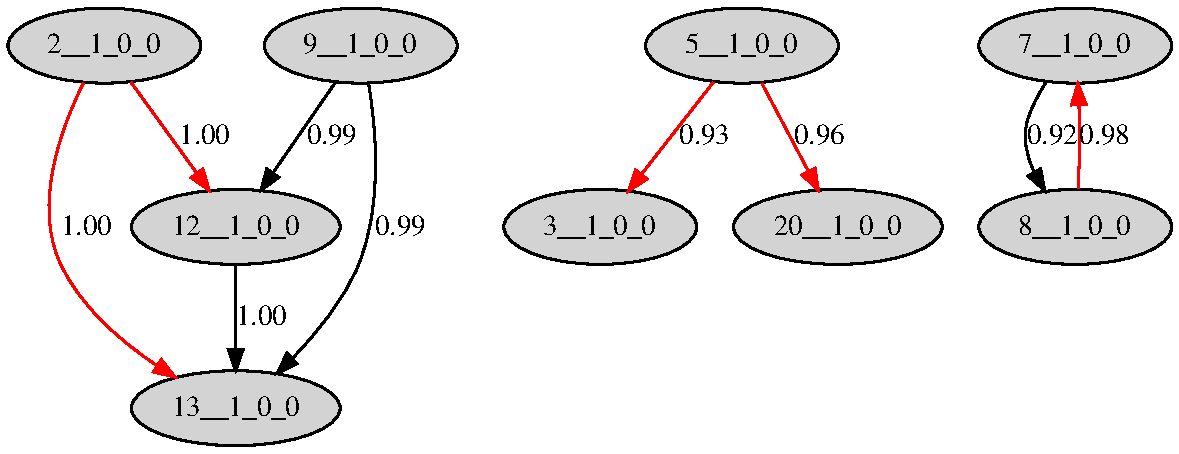
\includegraphics[width={0.9\linewidth}]{corr_graph_1.pdf}
  \caption{Correlation graph}
  \label{fig:ps:columncorrelation:corrgraph1}
\end{figure}

The main goal of the \nameref{subsubsec:ps:correlation} is to select a subset of the edges in the graph. We can define this process as the optimization problem of selecting a subset of edges in the correlation graph \(G\) such that the resulting subgraph \(G_{s}\) satisfies the following properties (in this order):
\begin{itemize}
    \item[\textit{P1}:] the indegree of any node is at most 1---a column should be determined by no more than 1 other column
    \item[\textit{P2:}] any path in \(G_{s}\) is of length 1---because of the transitivity property, for every path between nodes \(c_{a}\) and \(c_{b}\), there will also be a direct edge from \(c_{a}\) to \(c_{b}\)
    \item[\textit{P3}:] the number of nodes in \(G_{s}\) with indegree > 0 is maximal---the number of columns that are represented as functions of other columns is maximal
    \item[\textit{P4}:] the average weight of the edges is maximal---the edges with the highest correlation coefficient should be selected
\end{itemize}

We defined a Greedy algorithm for solving the correlation selection optimization problem. It builds the \(G_{s}\) graph by greedily selecting one edge at a time from \(G\). The edge is added to \(G_{s}\), \(G\) is updated and the process goes on until there are no more edges in \(G\). The algorithm is described in listings \ref{lst:ps:corr:selectcorr}, \ref{lst:ps:corr:nodescore}, \ref{lst:ps:corr:edgescore}.

\begin{lstlisting}[language=Python,
label={lst:ps:corr:selectcorr},
caption={select\_correlations}]
# G = correlation graph resulted from the correlation detection process
def select_correlations(G):
  G_s = <empty correlation graph>
  while G.edges is not empty:
    # select destination node
    dst = min(G.nodes, key=get_node_score)
    # select (_, dst) edge
    (src, dst, corr_coef) = min(dst.incoming_edges, key=get_edge_score)
    # update G_s
    G_s.add((src, dst, corr_coef))
    # update G
    G.remove(dst.incoming_edges)
    G.remove(dst.outgoing_edges)
    G.remove(dst)
    G.remove(src.incoming_edges)
  return G_s
\end{lstlisting}

\begin{lstlisting}[language=Python,
label={lst:ps:corr:nodescore},
caption={get\_node\_score}]
def get_node_score(node):
  indegree_src = min([src.indegree 
                     for (src, dst) in node.incoming_edges])
  return (node.outdegree, indegree_src, node.indegree)
\end{lstlisting}

\begin{lstlisting}[language=Python,
label={lst:ps:corr:edgescore},
caption={get\_edge\_score}]
def get_edge_score((src, dst, corr_coef)):
  return (src.indegree, -corr_coef, -src.out_degree)
\end{lstlisting}
\bigskip

Every iteration of the \textit{while} loop first selects the destination node of the candidate edge based on its score. The \textit{get\_node\_score} function prioritizes nodes with the minimum outdegree---ideally 0---such that the number of discarded edges as an effect of constraint \textit{P2} is minimized. The difference between nodes with the same outdegree is made by the minimum indegree of its parent nodes (source nodes of incoming edges)---for the same reason. Finally the difference is further made by the smallest indegree of the node itself, prioritizing columns with fewer options of being represented as functions of other columns. 

With the destination node fixed, the best edge is selected from its incoming edges. The \textit{get\_edge\_score} function prioritizes edges that have a minimum indegree---ideally 0---such that nodes at the start of correlation paths are selected. The difference between these nodes is further made based on the highest correlation coefficient and then by the highest outdegree.

The selected edge is added to \(G_{s}\) and \(G\) is updated such that constraints \textit{P1} and \textit{P2} are satisfied: the destination node, its incoming and outgoing edges and the incoming edges of the source node are removed. This process changes the degree of the nodes in \(G\) and impacts their scores.

The complexity of the algorithm, as described above, is given by the number of nodes in \(G\) and their average indegree: \(N^2 \times avg(indegree)\), where \(N\) is the number of nodes. Every iteration of the \textit{while} loop selects one node from \(G\) by computing the score of all nodes. The \textit{get\_node\_score} function loops through all incoming edges of the node. If the selection of the \(dst\) node is done with a priority queue the complexity is improved: \(N \times \log(N) \times avg(indegree)\).

An alternative approach would be to relax constraint \textit{P2} and allow paths of length higher than 1. Then apply a variation of the Dijkstra's shortest paths algorithm to shorten these paths with the goal of minimizing the complexity of the graph without affecting its average correlation coefficient. However, relaxing  \textit{P2} imposes a new constraint on \(G_{s}\): it should not contain any cycles. We leave this approach for future work.

% ---------------------------------------------------------------------------
% ----------------------- end of thesis sub-document ------------------------
% ---------------------------------------------------------------------------

\subsection{Iterative greedy learning}
\label{sub:learning:iterative}


% ----------------------- paths to graphics ------------------------



% ----------------------- contents from here ------------------------
% 

This section presents a greedy iterative algorithm for compression learning. It uses a pattern selector (\(S\)) to greedily choose how to compress columns (\ref{sub:learning:selectors}~\nameref{sub:learning:selectors}) and the pattern detectors (\(P\)) defined in \ref{sec:pd}~\nameref{sec:pd}. The algorithm takes a breadth-first approach, thus supporting pattern detectors \(P\) that work on multiple columns (e.g. \nameref{subsec:pd:columncorrelation}). It takes as input the list of input columns (\(c_{in}\)) and builds the compression tree one level at a time.

% https://en.wikipedia.org/wiki/Iterated_function
The algorithm builds the compression tree \(T\) in an iterative process. Let \textit{add\_level(\(T\))} be an iterated function which adds 0 or more expression nodes (\(N\)) on a new level in \(T\). This function is repeatedly applied to T in an iterative process. Each call of the function uses the updated version of \(T\) that it produced in the previous iteration. The iterative process converges to the final compression tree \(T_{out}\) once no more changes are made to \(T\) in an iteration.

The learning algorithm starts with \(P_{list}\) (a list of pattern detector instances), \(S\) (a pattern selector) and \(T\) (an empty compression tree, initialized with the list of input columns \(c_{in}\)). Recall that the compression tree is actually a graph with multiple connected components where each component is a directed acyclic graph with one or more root nodes (see \ref{sec:exprtree}~\nameref{sec:exprtree}). An additional parameter is \(it_{max}\), representing the maximum number of iterations. \(it_{max}\) also determines the maximum height of the compression tree (\(h_{max}\)), since every iteration adds a new level to \(T\).

The \textit{add\_level} function adds new compression nodes (\(N\)) to \(T\) by trying to further compress its leaf (output) columns \(c_{leaf}\). It does this in 2 steps. Step-1 pattern detection: use the pattern detectors \(P_{list}\) to generate all possibilities to compress the leaf columns, resulting in a list of expression nodes \(N_{list}\). Step-2 pattern selection: use the pattern selector \(S\) to select a subset of \(N_{list}\) (\({N_{s}}_{list}\)), representing the best way to compress each \(c_{leaf}\). Finally, the expression nodes in \({N_{s}}_{list}\) are added to as a new level. If no expression nodes (\(N\)) are selected (i.e. \({N_{s}}_{list}\) is empty), then the iterative learning algorithm converged to the final compression tree \(T\).

The algorithm is described in listings \ref{lst:learning:iterativegreedy:build_T} and \ref{lst:learning:iterativegreedy:add_level}.

\begin{lstlisting}[language=Python,
label={lst:learning:iterativegreedy:naming},
caption={Naming conventions}]
c = column
P = pattern detector
S = pattern selector
T = compression tree
N = compression node
\end{lstlisting}

\begin{lstlisting}[language=Python,
label={lst:learning:iterativegreedy:build_T},
caption={build\_T (iterative greedy)}]
def build_T(c_in_list, P_list, S)
  # initialize T with the input columns
  T = CompressionTree(c_in_list)
  # iterative process
  for it in range(0, it_max):
    add_level(T, P_list, S)
    if <no changes made to T>:
      break
  # return final compression tree
  return T
\end{lstlisting}

\begin{lstlisting}[language=Python,
label={lst:learning:iterativegreedy:add_level},
caption={add\_level (iterative greedy)}]
def add_level(T, P_list, S):
  c_leaf_list = T.c_leaf_list
  # pattern detection 
  N_list = list()
  for P in P_list:
    N_p_list = P.evaluate(c_leaf_list)
    N_list.extend(N_p_list)
  # select expression nodes
  N_s_list = S.select(N_list)
  # stop if no expression nodes were selected
  if len(N_s_list) == 0:
    return
  # add selected expression nodes to T
  T.update(N_s_list)
\end{lstlisting}
\bigskip

The complexity of the algorithm is given by the total number of columns in the final compression tree multiplied by the effort spent on evaluating the pattern detectors on it and choosing the expression node that it will be compressed with:
\begin{equation}
\label{eq:learning:recursiveexhaustive}
    c_{in} \times (b) ^ {h_{max}} \times (p + p \times \mathit{avg}(n_{p}))
\end{equation}
where:
\begin{itemize}
    \item[] \(c_{in}\) = number of input columns
    \item[] \(b\) = branching factor of the compression tree (as defined in Equation \ref{eq:optimizationproblem:b})
    \item[] \(h_{max}\) = maximum height of the compression tree
    \item[] \(p\) = number of pattern detectors
    \item[] \(n_{p}\) = number of expression nodes returned by a pattern detector
\end{itemize}
In the worst case when the maximum number of iterations is reached, \(h_{max}\) becomes \(it_{max}\), thus the complexity is bounded by \(it_{max}\).

Regardless of the nature of the pattern selector \(S\), the algorithm is greedy, as it makes irreversible locally best choices which only depend on previously made choices. The breadth-first approach allows the use of multi-column pattern detectors, representing an advantage compared to the \nameref{sub:learning:recursiveexhaustive} algorithm, which misses compression opportunities by handling each column separately. The greedy model significantly reduces the number of solutions explored, leading only to a locally best solution. At the same time, the reduced dimension of the explored solution set ensures faster termination of the algorithm. The advantages of both algorithms can be combined with the \nameref{sub:learning:multistage} approach described in section \ref{sub:learning:multistage}.

TODO-1: image describing the iterative process

% ---------------------------------------------------------------------------
% ----------------------- end of thesis sub-document ------------------------
% ---------------------------------------------------------------------------

\subsection{Recursive greedy learning}
\label{sub:learning:recursivegreedy}

% \iffalse
\begin{verbatim}
TODO
\end{verbatim}
% \fi

\iffalse
TODO-1-1: result: worse than iterative learning since it misses multi-column opportunities
TODO-1-2: advantage: faster execution (one column at a time; suitable for columnar storage)
TODO-2: comparison with the other algorithms & improvements brought to OR by them
\fi

\subsection{Multi-stage learning}
\label{sub:learning:multistage}

% ----------------------- paths to graphics ------------------------



% ----------------------- contents from here ------------------------
% 

\iffalse
\begin{verbatim}
- separate pattern detectors into groups (stages) based on rules that determine which patterns work good together
- use different pattern selector for each group
- instead of putting all the patterns together with only one selector
- each stage can take either the iterative approach or the recursive one
\end{verbatim}
\fi

We observed that each learning algorithm has advantages and disadvantages and works better with different types of pattern detectors. E.g. the \nameref{sub:learning:recursiveexhaustive} algorithm has a wide coverage of the solution space of the problem, but does not support multi-column pattern detectors. In contrast, the \nameref{sub:learning:iterative} algorithm does not miss multi-column compression opportunities and converges faster, but has a poor coverage of the solution space. Moreover, in the case of \nameref{sub:learning:iterative}, each pattern selector (\(S\)) is suitable for certain pattern detectors.

These observations lead to the conclusion that there is no \textit{one size fits all} learning algorithm and call for a combined approach that leverages the advantages of each of them. Therefore, we defined the \nameref{sub:learning:multistage} approach, which improves the learning process by chaining different algorithm instances together, each running in a separate stage.

An algorithm instance \(A(\mathit{args})\) is an application of algorithm \(A\) on the input parameters \(\mathit{args}\). E.g. \(\mathit{IG}(P_{1})\) and \(\mathit{IG}(P_{2})\) will produce different compression trees \(T_{1}\) and \(T_{2}\) even though they are both instances of the \nameref{sub:learning:recursiveexhaustive} algorithm, because the pattern detector lists that they use \(P_{1}\) and \(P_{2}\) differ. This abstraction allows us to run the same learning algorithm with different pattern detectors or selectors and combine their results.

Chaining compression learning algorithm instances \(A_{1}\) and \(A_{2}\) means executing \(A_{1}\) to get the compression tree \(T_{1}\), then executing \(A_{2}\) to build \(T_{2}\) based on \(T_{1}\). Chaining \(A_{1}\) and \(A_{2}\) requires that the output of \(A_{1}\) can be converted to the input of \(A_{2}\). This condition can be satisfied as all compression learning algorithms we proposed have compatible input and output parameters. The input of a learning algorithm is either one or more input columns or a compression tree. The output of all the algorithms is a compression tree. If \(A_{2}\) requires a compression tree as input, then \(T_{1}\) can be passed directly to it. If \(A_{2}\) requires a list of columns, then the leaf columns of \(T_{1}\) are passed to \(A_{2}\). In the second case, the output of \(A_{2}\) (\(T_{2}\)) needs to be merged with \(T_{1}\) to form the final compression tree \(T_{out}\). Additional input parameters (pattern detectors (\(P\)), pattern selectors (\(S\)), estimators (\(E\))) are independent of the result of the previous algorithm.

This generic multi-stage design allows easy experimentation with any combination of compression learning algorithm instances. One example of chaining 2 learning algorithms is the following: first execute an instance of \nameref{sub:learning:recursiveexhaustive} with the single-column pattern detectors. Then execute an instance of \nameref{sub:learning:iterative} with the multi-column pattern detector \nameref{subsec:pd:columncorrelation} and the \nameref{subsubsec:ps:correlation}. This will result in building the best compression tree using single-column pattern detectors and then identifying and exploiting correlations between the leaf columns of the tree, irrespective of their type (exceptions or not). While this setup misses correlation opportunities between intermediate/internal columns, it led to complex correlation graphs that considerably reduce the number of physical columns---we present these results in \ref{subsec:eval:results:recursiveexhaustive} and Appendix~\ref{appendix:corrgraphs}.

% This generic multi-stage design allows easy experimentation with any combination of compression learning algorithm instances, but this setup, in particular, led to good results which we present in \ref{subsec:eval:results:recursiveexhaustive}.

% TODO-1: diagram showing the multi-stage algorithm chaining

% ---------------------------------------------------------------------------
% ----------------------- end of thesis sub-document ------------------------
% ---------------------------------------------------------------------------

% ---------------------------------------------------------------------------
% ----------------------- end of thesis sub-document ------------------------
% ---------------------------------------------------------------------------